
\section{PCL}
\noindent   PCL je samostný, vysoko škalovateľný, otvorený projekt pre 2D a 3D obrázky a spracovávanie point cloud. Knižnica je cross platform, napisana v jazyku C++ a Pythone. Najčastejšie sa použiva na operačnom systéme Linux. Existujú package aj pre macOS a Windows vytvorené tretímy stranami. My v tomto projekte budeme používať Ubuntu 22.04. LTS a verzia PCL je  1.12.1. Knižnica ja vydana pod BSD licenciami čo znamená, že je voľne použiteľna úre komerčné účely a za účelom výskumu.
\acrfull{ransac} je dlhá skratka naopak \acrshort{nn} je skratka v krátkej forme.\acrshort{pcl} je skratka v krátkej forme.

\subsection{Inštalácia PCL}
PCL je dostupný na mnoho distribúcii Linuxu ako Ubuntu, Debian, Fedora, Gentoo a Arch Linux. PCL na distribúciach Ubuntu a Debian môžeme nainštalovať pomocou.

sudo apt install libpcl-dev

Na Windowse sa PCL inštaluje pomocou vpckg package manažéra vytvoreného Microsoftom. 

PS> .\vcpkg install pcl

MacOS ma Homebrew package manažéra ktorý podporuje inštaláciu packagov, ktoré Apple alebo Linux nedokáže nainštalovať. 
brew install pcl
Toto su odporúčane inštalacie pre PCL na daných operačných systémoch.

\subsection{Používanie PCL}
Na používanie PCL si potrebujeme v našom kóde vložiť potrebné knižnice. Po nainštalovaní sa v našom systéme nastavia premenné, takže stači nám použiť príkaz v C++, #include <pcl/“názov_knižnice“.h>.
\subsection{Kompilácia projektu}
Vytvoríme si súbor CMakeList.txt v ktorom zadefinujeme potrebné premenné aby make vedel najsť cestu ku knižnici a vedel aké súbory ma skompilovať. Ďalej vytvoríme priečinok s názvom build, v terminály vojdeme do neho a pomocou príkazu cmake “cesta k CMakeList.txt“, si vytvorime makefile. Ďalej používame len príkaz make ktorý nam vytvorí súbor pomocov ktorého môžeme spustiť projekt.
\section{Point Cloud}
\subsection{General}
Je to súbor bodov v priestore. Body môžu reprezentovať 3D tvary alebo objekty. Každý bod má karteziánske súradnice (X,Y,Z). Point cloud je generovaný pomocou 3D skenera alebo pomocou softwaru na fotogrametriu, ktorý meria veľa bodov na externom povrchu objektov okolo. My v tomto projekte použijeme Kinect 2 (odsek 6). Point cloud sa používa v 3D modelovaní, metrológii, meranie kvality výrobkov a rôzne vizualizácie. Point cloud sa často zarovnáva s 3D modelmi alebo inými point cloudmi ako registrácia množín bodov.
\subsection{Pouzitie}
Pre priemyselnú metrológiu alebo inšpekciu pomocou priemyselnej počítačovej tomografie možno mračno bodov vyrobeného dielu zosúladiť s existujúcim modelom a porovnať, aby sa skontrolovali rozdiely. Geometrické rozmery a tolerancie možno získať aj priamo z point cloudu.
\subsection{Konverzia do 3D povrchu}
V geografických informačných systémoch sú point cloudi jedným zo zdrojov využívaných na tvorbu digitálneho výškového medelu terénu. Používajú sa aj na generovanie 3D modelov mestského prostredia. Drony sa často využívaju na nazbieranie RGB obrázkov ktoré sa neskôr pomocov algoritmu strojového videnia ako je AgiSoft Photoscan, PixčD alebo DroneDeploy používaju na vytvorenie RGB point cloudu, kde sa môže požiť vzdialenostná a objemová aproximácia.
\section{RANSAC}
\subsection{Overview}
RANSAC je algoritmus vytvorený Fischlerom a Bollesom, určuje všeobecný prístup k odhadu parametrov, s veľkym podielom outliers v stupnom datasete. Na rozdiel od iných výkonných algoritmov odhadu, ako napríklad M-estimators a meródov najmenších štvorcov s prepojením na strojové učenie. RANSAC bol vytváraný komunitov ľudi používajúci strojové učenie. RANSAC je vzorkovacia technika ktorá generuje kandidáta na minimalny pocet pozorovani potrebnych na zistenie odhadu parametrov leziacich pod modelom. Narozdiel od ostatných vzorkovacích algoritmov, ktoré používaju čo najviac bodov ako môžu, RANSAC používa najmenši počet bodov ako môže.
\subsection{Algoritmus}
\begin{enumerate}
    \item Vybranie minimum náhodných bodov potrebných na určenie parametrov modelu
    \item Vyriešenie parametrov pre model
    \item Určenie koľko bodov z množiny všetkých bodov leží s preddefinovanou ε.
    \item Ak zlomok bodov ležiacich v preddefinovanej ε, presahuje preddefinovaný prah τ, prehodnotí parametre modelu použitím všetkých identifikovaných inliers a ukonči.
    \item Inak, opakuj kroky 1 až 4, s maximálnym N opakovaniami.
\end{enumerate}
\begin{figure}[!htbp]
  \centering
  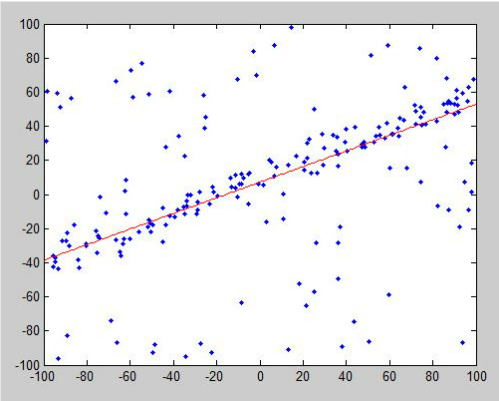
\includegraphics[width=8cm]{img/ransac2D.png}
  \caption{Priklad algoritmu v 2D rovine}
  \label{vzhladobr}
\end{figure}
Modre sú body z datasetu, pomocou RANSAC algoritmu sa určili 2 body, ktoré majú vo svojom subsete najmenej bodov ležiacich mimo alfy.
\subsection{RANSAC 3D}
Podobne ako pri opise vyššie RANSAC 3D funguje s výberom náhodnych troch bodov na ktorých zostaví rovinu a spočita body ležiace v rovine a body ležiace mimo roviny. Algoritmus sa opakuje n-opakovaní a výstupom je najlepší model.
\subsection{Neural guided RANSAC}
\section{KINECT}
Kinect je vstupné zariadenie snímajuce pohyb, vyrobené Microsoftom. Zariadnei obsahuje RGB kamery a infračervený projektor a detektor ktorý monitoruje hĺbku priestoru na zaklade štrukturovateľného svetla alebo na zaklade času trvajúcemu svetlu dopadnuť na objekt, vďaka ktorému vie kinect poskytnúť rekognizáciu giest v reálnom čase. Kinect sa použiva hlavne v hernom priemysle, ale používa sa taktiež na komerčné a akademické učely pretože poskytuje mapovanie priestoru a je lacnejši než profesionálne zariadenia.  
\subsection{Ako funguje}
Infračervený projektor na kinevte posiela modulované infračervené svetlo ktoré je zachytené sensormy. Infračervené svetlo ktoré sa odrazí od bližších objektov ma kratší čas letu ako svetlo ktoré sa odrazí od vzdialenejších objektov, takže sensor sníma ako vymodulovaný vzor bol deformovaný z času letu svetla, pixel po pixeli. Čas príletu meranej hlbky touto metódov môže byť presnejšie vypočítany v kratšom čase, čo zabezpečí viac snímkov za sekundu. Hneď ako kinect naskenuje hlbkovú fotografiu, použije metódu zisťovania hrán k vytýčeniu bližších objektov z pozadia fotky. 
\section{Implementavanie RANSAC algoritmu}
\section{Vystupy}
\section{Implementovanie RANSAC alfgoritmu s pouzitim NN}
\section{Zaver}

\begin{lstlisting}[
  caption={Ukážka algoritmu},
  label={lst:main-c},
  language=c
]
/* Hello World program */

#include<stdio.h>

struct cpu_info {
    long unsigned utime, ntime, stime, itime;
    long unsigned iowtime, irqtime, sirqtime;
};

main()
{
    printf("Hello World");
}
\end{lstlisting}